\Chapter{VueJS implementáció}

CRUD műveletek megvalósítása a services/FightersService.js fájlban:

\begin{cpp}
export default {
  fetchFighters () {
    return Api().get('fighters')
  }, 
  addFighter (params) {
    return Api().post('fighters', params)
  },
  updateFighter (params) {
    return Api().put('fighters/' + params.id, params)
  },
  getFighter (params) {
    return Api().get('fighter/' + params.id)
  },
  deleteFighter (id) {
    return Api().delete('fighters/' + id)
    this.fetchFighters();
  }
}
\end{cpp}

A fetchFighters nevezetű függvény visszaadja az Api().get(’fighters’) kérést, amit az axios modul végez el, ami egy promise alapú http kliens. Ehhez szükséges importálni a FightersService.js fájlban a services/Api.js fájlt, ami biztosítja az axios modult.

\begin{cpp}
import Api from '@/services/Api'
\end{cpp}

A getFighter(), és az updateFighter() függvények az URL címből veszik át a harcos id-ját.

A deleteFighter() függvény pedig miután megkapta az id-t, meghívja a fetchFighters() nevű függvényt, ami újra lekéri az aktuálisan eltárolt harcosokat.

Api.js

\begin{cpp}
import axios from 'axios'
export default() => {

  return axios.create({
    baseURL: `http://localhost:8081`
  })
}
\end{cpp}

\Section{Routing}

Szükséges hozzá importálnunk a vue-router-t és használni:

\begin{cpp}
import Router from 'vue-router'
\end{cpp}

Majd a routing-ok (útvonalak) megadásánál a Vue.use(Router) sorral adjuk meg, hogy a program használja Router-ként a beimportált „vue-router” nevezetű modult.

\begin{cpp}
export default new Router({
mode: 'history',
  routes: [
{
      path: '/fighters',
      name: 'Fighters',
      component: Fighters
  },
  {
      path: '/fighters/new',
      name: 'NewFighter',
      component: NewFighter  }]})
\end{cpp}

Az alapvető beállítás a vue-router modulban az úgynevezett „hash mode”, ami az URL hash-t (\#) használja a teljes URL cím reprezentálására, így ha az URL változik, az oldal nem fog újra lefrissülni.

A mode: ’history’ használatával a vue-router-t „history mode”-ban használhatjuk, amivel megszabadulhatunk a hash-től az URL címekben. Ez a mód arra használja a history.pushState API-t, hogy elérje, hogy a felhasználó navigálhasson az URL-ek között, anélkül, hogy az oldal újra lefrissülne. Ehhez megfelelő szerver konfiguráció szükséges, különben a felhasználó egyes oldalak elérésekor 404-es hibaüzenetet kaphat.

A path definiálja az oldal URL címét, a component mutatja meg, hogy melyik .vue fájl tartalmát kell megjeleníteni az URL-re való látogatáskor. Ehhez a megadott komponenseket importálnunk kell.

\begin{cpp}
import Fighters from '@/components/Fighters'
import NewFighter from '@/components/NewFighter'
\end{cpp}

A /fighters/new URL megnyitásakor a NewFighter.vue komponens töltődik be, ami tartalmazza a megjelenítendő template-t, amiben egy új harcos létrehozásához szükséges form található.

\Section{Form validáció}

A form validálást többféle módon történhet, az egyik ilyen a vee-validate nevezetű modul használatával történő validáció. Ehhez először telepíteni kell a modult npm csomagkezelő, vagy CDN segítségével, majd az alábbiakat kell importálni az alkalmazás main.js fájljában:

\begin{verbatim}
npm install vee-validate --save
import Vue from 'vue'
import VeeValidate from 'vee-validate'
Vue.use(VeeValidate)
\end{verbatim}

A name mező validálása:

\begin{verbatim}
<div class="form-group" :class="{'has-error': errors.has('name') }">
        <label for="Name">Name*</label>
          <input type="text" v-model="name" name="name" class="form-control" id="Name" placeholder="Name" v-validate="'required|alpha_spaces|min:3'"> 
<span v-show="errors.has('name')" class="text-danger">{{ errors.first('name') }}</span>
        </div>
\end{verbatim}

A v-validate input mezőhöz való hozzáadása után lehet megadni az úgynevezett szabályokat (rules), ez esetben required, alpha\_spaces és min:3, tehát a mező kitöltése kötelező, a felhasználónak csak alfabetikus karaktereket és közöket (space) lehet a mezőbe írnia, egyéb esetben a mező nem érvényes. A min:3 a minimum karakterszámot állítja be 3-ra.

A v-show direktíva használatával piros színű szegéllyel határolt mező jelenik meg, ha a mező értéke még nem valid (érvényes). Ha a felhasználó belekattint a mezőbe, majd kikattint belőle úgy, hogy nem írt a mezőbe semmit, akkor a program által előre definiált hibaüzenet jelenik meg: „The name field is required.”

Ezenkívül minden egyes szabályra is az előre meghatározott hibaüzenetek jelennek meg, ha a felhasználó numerikus karaktert ír be, vagy ha kevesebb mint a 3 karakter a begépelt szöveg hossza.

A szám mezők validációja hasonlóan történik:

\begin{verbatim}
<div class="form-group" :class="{'has-error': errors.has('height') }">
       	<label for="Height">Height*</label>
<input type="number" class="form-control" name="height" placeholder="Height" v-model="height" id="Height" v-validate="'required|min_value:155|max_value:205'">
<span v-show="errors.has('height')" class="text-danger">{{ errors.first('height') }}</span>
        </div>
\end{verbatim}

Itt a height mező értékét adhatjuk meg a min\_value és max\_value szabályokkal, ha a felhasználó nem 155 és 205 közötti számértéket ír be a mezőbe, akkor kiíródik a hibaüzenet.

A record mezőnél a
\begin{verbatim}
v-validate="'required|regex:^[0-9]+[-][0-9]+[-][0-9]+$'"
\end{verbatim}
megadása után a record mező csak akkor lesz érvényes, ha a felhasználó azt ilyen formában adja meg. Például: 100-10-1

Az image\_url mezőnél pedig a
\begin{verbatim}
v-validate="'required|regex:^https?://.+$'"
\end{verbatim}
megadása után a felhasználó csak érvényes URL linket adhat meg a harcos avatarjának.

A form fejlécében lévő @submit.prevent=”validateBeforeSubmit” arra szolgál, hogy mikor a felhasználó rákattint a Submit gombra, a form-ot a program még nem küldi el, csak miután meghívta a „validateBeforeSubmit” nevű függvényt.

\begin{verbatim}
<form @submit.prevent="validateBeforeSubmit">

validateBeforeSubmit() {
      this.$validator.validateAll().then((result) => {
        if (result) {
          // eslint-disable-next-line
          this.addFighter()
          return; }});
}
\end{verbatim}

Ez a függvény megnézi a validateAll() függvény eredményét, és ha minden mező érvényes, akkor meghívja az addFighter() függvényt, ami a FightersService nevű szervízben van definiálva. Ekkor ha a felhasználó a Submit gombra kattint, az összes hibaüzenet azonnal megjelenik, de az addFighter() függvény még nem hívódik meg.

A NewFighter komponens tartalmaz egy <template></template> tagok közötti részt, amiben a megjelenítendő template-t tudjuk megadni. 

A <script></script> tagok között adhatjuk meg a szükséges függvényeket, metódusokat, funkciókat.

Ehhez importálnunk kell a FighterService-t:

\begin{cpp}
import FightersService from '@/services/FightersService'

export default {
  name: 'NewFighter',
  data () {
    return {
      name: ' ',
      nickname: ' ' }}
\end{cpp}

A data részben a form-ból átvett mezőknek az értékét állítjuk be egy üres sztring-re.
Majd a methods résznél megadjuk, hogy a FighterService-ben lévő addFighter függvény pontosan mit hajtson végre:

\begin{cpp}
methods: {
    async addFighter () {
      await FightersService.addFighter({
        name: this.name,
        nickname: this.nickname
      })
      this.$router.push({ name: 'Fighters' })
    }
\end{cpp}

A form mezőiben megadott adatokkal tölti fel a megfelelő mezőket, ezután a függvény megkapja a megfelelő paramétereket és az Api szerviz az axios modulon keresztül egy HTTP POST kéréssel hozzáadja a fighters objektumot az adatbázishoz.

\begin{cpp}
addFighter (params) {
    return Api().post('fighters', params)}
\end{cpp}

A megjelenítendő harcosok szűrése
Szükséges hozzá egy beviteli mező:

\begin{verbatim}
<div class="search">
<input type="text" style="text-align:center;" v-model="search" placeholder="Search fighters..."/>
</div>
\end{verbatim}

Továbbá a <script></script> tagok között a data () részben definiálnunk kell egy a „search” nevezetű mezőt.

\begin{cpp}
export default {
  name: 'fighters'
   data () {
    return {
      fighters: [],
      search:' '  }},
computed: {
    	filteredFighters: function(){
    		return this.fighters.filter((fighter) => {
return fighter.name.toLowerCase().match(this.search.toLowerCase());
    		});}}
}
\end{cpp}

Ezután a filteredFighters() függvény-ben a fighters objektumban lévő fighter-eket szűrjük a .filter kulcsszóval, és ha a harcos „name” mezőjének kisbetűs formára alakított változata megegyezik a „search” nevű beviteli mezőbe beírt érték kisbetűs formára alakított változatával, akkor csak azok a harcosok maradnak a táblázatban, amelyek neve tartalmazza a search mezőbe beírt karaktert, vagy karaktersorozatot.

Ha toLowerCase() függvény alkalmazása mind a name, mind a search mezőre biztosítja, hogy ha a felhasználó kisbetűvel is kezdi a beírt értéket, a program a nagybetűvel kezdődő neveket is benne hagyja a táblázatban.

Ezután a <table> <tbody></tbody> tag-jai között a filteredFighters nevű listán megy végig a ciklus, és jeleníti meg a harcosok adatait, a „search” mező segítségével pedig a beírt érték alapján szűrhetjük a megjelenítendő harcosokat.

\begin{verbatim}
<tbody>
        <tr v-for="fighter in filteredFighters">
          <td>{{ fighter.name }}</td>
          <td>{{ fighter.nationality }}</td>
        </tr>
 </tbody>
\end{verbatim}

\Section{Projekt struktúra}

\begin{figure}[htb]
\centering
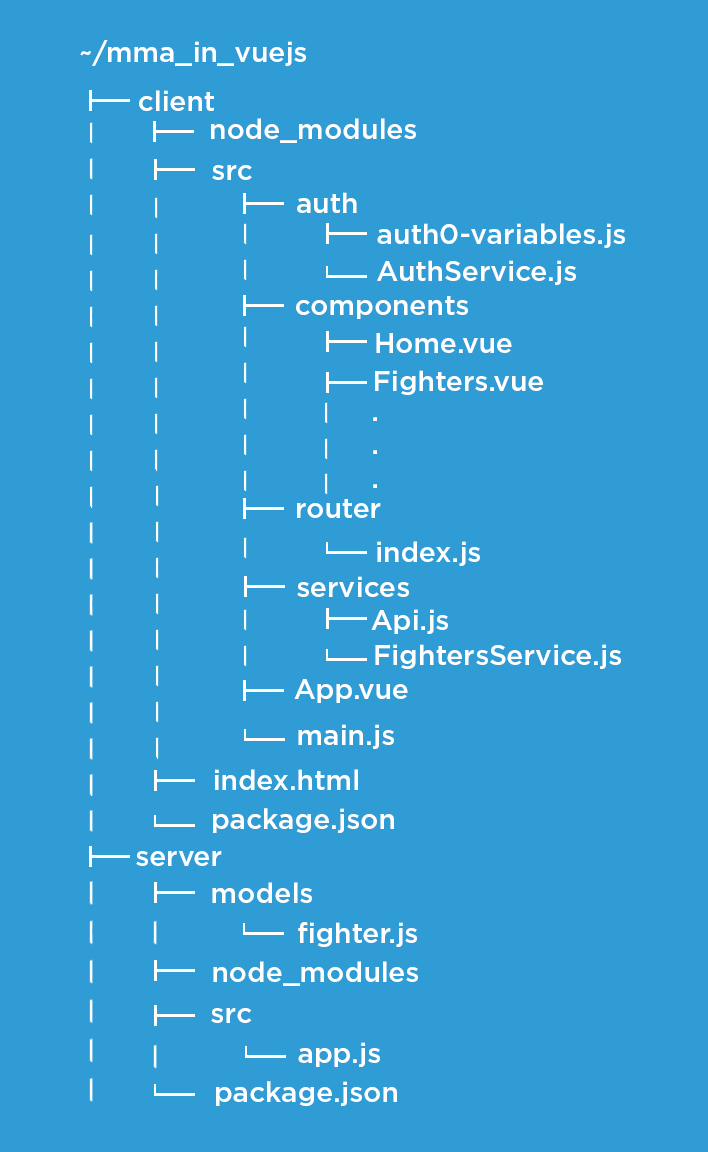
\includegraphics[scale=0.4]{kepek/mma_in_vue.jpeg}
\caption{A Vue.js projekt struktúrája}
\label{fig:vue_structure}
\end{figure}
